\documentclass[10pt]{article}
\usepackage[utf8]{inputenc}
\usepackage[T1]{fontenc}
\usepackage[vietnamese]{babel}
\usepackage{a4wide,amssymb,epsfig,latexsym,multicol,array,hhline,fancyhdr}
\usepackage{lastpage}
\usepackage{enumerate}
\usepackage{xcolor}
\usepackage{graphicx}
\usepackage{array}
\usepackage{tabularx}
\usepackage{multirow}
\usepackage{multicol}
\usepackage{rotating}
\usepackage{graphics}
\usepackage{hyperref}
%\usepackage[hidelinks]{hyperref}
\usepackage{setspace}
\usepackage{epsfig}
\usepackage{tikz}
\usepackage{placeins}
\usepackage{appendix}
\usepackage{booktabs}
\usepackage[head=30pt,a4paper,top=30mm,bottom=30mm]{geometry}
\usetikzlibrary{arrows,snakes,backgrounds}

\usepackage{listings}
\usepackage{textcomp}
\definecolor{listinggray}{gray}{0.9}
\definecolor{lbcolor}{rgb}{0.9,0.9,0.9}
\lstset{frame=tb,
  language={[Visual]Basic},
  aboveskip=3mm,
  belowskip=3mm,
  showstringspaces=false,
  columns=flexible,
  basicstyle={\small\ttfamily},
  numbers=none,
  numberstyle=\tiny\color{gray},
  keywordstyle=\color{blue},
  commentstyle=\color{green},
  stringstyle=\color{orange},
  breaklines=true,
  breakatwhitespace=true
  tabsize=3
}




\newcolumntype{L}[1]{>{\raggedright \arraybackslash}p{#1}}
\newcolumntype{C}[1]{>{\centering   \arraybackslash}p{#1}}

\newtheorem{theorem}{{\bf Theorem}}
\newtheorem{property}{{\bf Property}}
\newtheorem{proposition}{{\bf Proposition}}
\newtheorem{corollary}[proposition]{{\bf Corollary}}

\newif\ifshortversion
\shortversiontrue 	% hide this line when shortversion==false
\newcommand\version[2]{\ifshortversion #1 \else #2 \fi}
\newcommand{\specialcell}[2][c]{%
	\begin{tabular}[#1]{@{}c@{}}#2\end{tabular}}
%\usepackage{fancyhdr}
\setlength{\headheight}{40pt}
\pagestyle{fancy}
\fancyhead{} % clear all header fields
\fancyhead[L]{
 \begin{tabular}{rl}
    \begin{picture}(25,15)(0,0)
    \put(0,-8){
\includegraphics[width=8mm, height=8mm]{hcmut.png}}
    %\put(0,-8){\epsfig{width=10mm,figure=hcmut.eps}}
   \end{picture}&
	%
\includegraphics[width=8mm, height=8mm]{hcmut.png} & %
	\begin{tabular}{l}
		\textbf{\bf \ttfamily Trường Đại Học Bách Khoa Tp.Hồ Chí Minh}\\
		\textbf{\bf \ttfamily Khoa Khoa Học và Kỹ Thuật Máy Tính}
	\end{tabular} 	
 \end{tabular}
}
\fancyhead[R]{
	\begin{tabular}{l}
		\tiny \bf \\
		\tiny \bf 
	\end{tabular}  }
\fancyfoot{} % clear all footer fields
\fancyfoot[L]{}
\fancyfoot[R]{\ttfamily Trang {\thepage}/\pageref{LastPage}}
\renewcommand{\headrulewidth}{0.3pt}
\renewcommand{\footrulewidth}{0.3pt}

\def\x86{80x86 }
\def\mips{MIPS }

%%%%%%%%%%%%%%%%%%%%%%%%%%%%%%%%%%%%%%%%%%%%%%%%%%%%%%%%%%
\begin{document}
	
	\begin{titlepage}
		\begin{center}
			ĐẠI HỌC QUỐC GIA THÀNH PHỐ HỒ CHÍ MINH \\
			TRƯỜNG ĐẠI HỌC BÁCH KHOA \\
			KHOA KHOA HỌC VÀ KỸ THUẬT MÁY TÍNH 
		\end{center}
		
		\vspace{0.7cm}
		
		\begin{figure}[h!]
		\begin{center}
		
\includegraphics[width=5cm]{hcmut.png}
		\end{center}
		\end{figure}
		
		\vspace{0.3cm}		
		
		\begin{center}
			\begin{tabular}{c}
				\multicolumn{1}{l}{\textbf{{\Large MẠNG MÁY TÍNH}}}\\
				\\
				\hline
				\\
				\multicolumn{1}{l}{\textbf{{\Large Assignment 1}}}\\
				\\
				\textbf{{\Huge $Love Is...$ - Ứng dụng chat qua mạng}}\\
				\\
				\hline
				\\
			\end{tabular}
		\end{center}
		
		\vspace{1.7cm}
		
		\begin{minipage}[t]{0.550\linewidth}
			\textbf{GVHD}: \\
			\ Thầy Nguyễn Hồng Nam
		\end{minipage}
		\begin{minipage}[t]{0.3\linewidth}
			\textbf{Nhóm Fight:}\\
			1. Nguyễn Văn Đức\\
			2. Vũ Thành Công\\
			3. Nguyễn Đức Thọ\\
		\end{minipage}
		\begin{minipage}[t]{0.20\linewidth}
			\textbf{}\\
			- 1410953\\
			- 1410413\\
			- 1413817
		\end{minipage}
		
		\vspace{1cm}
		
		\begin{center}
			\Large \today
		\end{center}
	\end{titlepage}
	
	\newpage


	\newpage
	
	\tableofcontents
	
	\newpage
	
	\section{Chức năng của ứng dụng}
		\begin{itemize}
			\item Tạo, đăng nhập tài khoản \\\\
			Người dùng có thể nhanh chóng tạo cho mình tài khoản để tham gia chat với bạn bè cùng sử dụng ứng dụng.
			\item Hiển thị danh sách bạn bè hiện có, đang online, offline\\\\
			Người dùng dễ dàng quản lý được bạn bè mình đang online để thực hiện chat giữa hai người, chat nhóm,… trong danh sách bạn bè mình đang có.
			\item Thêm bạn\\\\
			Chỉ cần biết tên tài khoản của ai đó, chỉ với vài bước đơn giản, người dùng có thể chat với người ấy dễ dàng.
			\item Chat giữa hai người\\\\
			Chọn tên người bạn trong danh sách bạn bè của bạn và chat ngay lập tức hoặc có thể gửi tin nhắn, file,… cho người đang offline và người đó sẽ nhận được tin nhắn,file,.. đó khi online.
			\item Chat đồng thời\\\\
			Bạn có thể cùng lúc chat với nhiều người qua nhiều cửa sổ khác nhau.
			\item Chat nhóm\\\\
			Bạn và bạn bè của bạn có thể chat chung với nhau qua một cửa sổ và mọi người đều thấy được tin nhắn của người khác.
			\item Gửi file qua lại khi chat\\\\
			Ngoài tin nhắn văn bản thông thường thì bạn có thể gửi và nhận file bất kì thông qua ứng dụng này. Bạn có thể vừa chờ upload file vừa tiếp tục chat với bạn bè.

		\end{itemize}
		
	\section{Thiết kế ứng dụng}
		\subsection{Mô hình tương tác}
			Mô hình Client-Server, sử dụng giao thức WebSocket.
			\begin{itemize}
				\item Nhóm chọn mô hình Client-Server. Server có thể quản lý, phân luồng dữ liệu trao đổi giữa các Client. Ngoài ra, Server còn kiểm tra, đảm bảo tính an toàn, toàn vẹn của dữ liệu khi nhận và khi gửi, thực hiện việc lưu dữ liệu vào database. Nhờ vậy, ta có thể quản lý, back up được dữ liệu, đồng thời đảm bảo khả năng dữ liệu được gửi đến Client nhận cao nhất.
				\item WebSocket là công nghệ hỗ trợ giao tiếp hai chiều giữa Client và Server bằng cách sử dụng một TCP socket để tạo một kết nối hiệu quả, ít tốn kém, có độ trễ thấp và dễ xử lý lỗi. Hỗ trợ giao tiếp hai chiều tức là Client và Server luôn nhận dữ liệu mới theo thời gian thực (2 chiều: server đến client hoặc client đến server).
			\end{itemize}
		
		\subsection{Database}
			Nhóm sử dụng hệ quản trị cơ sở dữ liệu MySQL. MySQL dễ sử dụng, hiệu suất cao, chi phis thấp. Ngoài ra MySQL còn hỗ trợ JSON, một định dạng hoán vị dữ liệu nhanh, trao đổi dữ liệu độc lập, với các built-in function cho phép lưu trữ, tìm kiếm.\\\\
			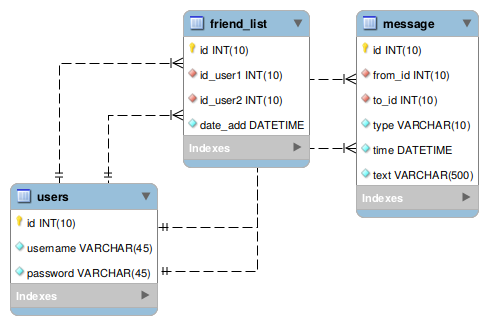
\includegraphics{erd.png}
			
		\subsection{Protocol}
			Nhóm sử dụng JSON để định dạng dữ liệu gửi đi và nhận về từ client.\\
			Trong các message gửi đi hay nhận về, đều có một trường $type$ nhằm xác định loại message để dễ dàng phân loại và xử lý.\\\\

			\begin{tabular}{l|l}
			\hline 
			$userRegReq$ & Client gửi Request yêu cầu tạo một user account mới \\ 
			\hline 
			$userLoginReq$ & Client gửi Request yêu cầu kiểm tra thông tin và đăng nhập \\ 
			\hline 
			$userRes$ & Server trả về Response trả lời cho Request yêu cầu đăng ký hoặc đăng nhập \\ 
			\hline 
			$text$ & Client/Server gửi text message cho nhau \\ 
			\hline 
			$file$ & Truyền và nhận file \\ 
			\hline 
			$userUpdate$ & Server gửi các thông tin về bạn bè của user mỗi khi có thay đổi, realtime \\ 
			\hline 
			$error$ & Server gửi lỗi về Client \\ 
			\hline 
			\end{tabular} 
			\subsubsection{Tạo kết nối}
			Client phải gửi một WebSocke handshake request đến Server. Server sẽ gửi trả lại WebSocket handshake response. Client sẽ kiểm tra và thực hiện kết nối.
			\subsubsection{Đăng nhập/đăng kí}
				Đối với user mới, cần phải đăng ký để sử dụng được ứng dụng. Khi đó với thông tin user nhập vào, Client gửi một message lên Server có dạng như sau:\\\\
				\begin{lstlisting}
		{
			"type": "userRegReq",
			"username": "newuser",
			"password": "newuser"
			"fullname":"New User"
		}
		        	\end{lstlisting}
		        	Đối với user đã đăng ký rồi, chỉ cần nhập username và password để thực hiện đăng nhập.
				\begin{lstlisting}
		{
			"type": "userLoginReq",
			"username": "ten_dang_nhap",
			"password": "mat_khau"    
		}
	        		\end{lstlisting}
		        	Về phía Server khi nhận được dạng message trên, Server chỉ trả về một loại message sau nếu thành công. Nếu có lỗi, Server gửi message dạng $error$ về.
					\begin{lstlisting}
		{
			"type": "userRes",
			"friendList":
			[
				{
					"friendname":"vtcong", 
					"online": true
				},
				{
					"friendname":"nvduc",
					"online": false
				}
			]
		}
		        	\end{lstlisting}
			\subsubsection{Chat giữa hai user}
				Client gửi message sau
				\begin{lstlisting}
        {
	        "type": "text",
	        "messType": "peer",
	        "time": "yyyy-MM-dd HH:mm:ss",
	        "toFriend": "userNhan",
	        "text": "noi_dung_chat"
        }
        			\end{lstlisting} 
				Server nhận message trên, thực hiện việc lưu vào database đồng thời gửi về cho user nhận.
				\begin{lstlisting}
        {
	        "type": "text",
	        "time": "",
	        "messType": ""
	        "fromFriend": "userGui",
	        "text": "noi_dung_chat"
        }
                	\end{lstlisting}
    			\subsubsection{Truyền và nhận file}
    				Trước khi Client truyền file lên Server cần gửi một message để Server biết và chuẩn bị nhận file.
				\begin{lstlisting}
	    {
		    "type": "file",
		    "fileName": "fight.txt",
		    "fileSize": 1024,
		    "toFriend": "userNhan"
	    }
				\end{lstlisting}
				Nhận được message trên, Server gửi message sau cho user nhận
				\begin{lstlisting}
	    {
		    "type": "file",
		    "fileName": "fight.txt",
		    "fileSize": 1024,
		    "fromFriend": "userGui"
	    }
				\end{lstlisting}
				nếu user nhận đồng ý nhận file, Client gửi lên Server message sau
				\begin{lstlisting}
	    {
		    "type": "file",
		    "fileName": "fight.txt",
		    "fileSize": 1024,
		    "status": "ok"
	    }
				\end{lstlisting}
				nếu không đồng ý, trường $status$ có giá trị là $"no"$.
				Server gửi lại message trên về user gửi để đồng ý tiếp tục hoặc hủy việc truyền file. Việc truyền file được thực hiện bằng cách gửi từng byte dữ liệu của file.
    			\subsubsection{Update thông tin về bạn bè của user}
    				Server phát hiện các thay đổi về bạn bè của user(offline, online, thay đổi status,...), gửi về user để cập nhật realtime.
				\begin{lstlisting}
	    {
		    "type": "userUpdate",
		    "friendname":"",
		    "status": "",
		    "online": true/false
	    }
    				\end{lstlisting}
			\subsubsection{Thông báo lỗi}
				Khi phát hiện lỗi Server trả một message thông báo lỗi cho người dùng.
				\begin{lstlisting}
	    {
		    "type": "error",
		    "errorCode": 10,
		    "errorDescription": "Username/password is incorrect"
	    }
            		\end{lstlisting}
            		Một số mã lỗi:
            		\begin{center}
            		\begin{tabular}{l|l}
			\hline 
			$10$ & Registration failed. \\ 
			\hline 
			$11$ & The username or password for Love Is is incorrect. \\ 
			\hline 
			$12$ & This account has already been confirmed.\\
			\hline 
				\end{tabular}
            		\end{center}
	\section{Triển khai ứng dụng}
		\subsection{Phía server}
		Server được hiện thực theo ý tưởng của mô hình 3 lớp, có thay đổi để phù hợp với ứng dụng.
			\begin{itemize}
				\item Presentation Layer: gồm class LoveIsServer, thực hiện việc giao tiếp với client, gửi và nhận các message, kiểm tra message do client gửi lên.
				\item Business Logic Layer: gồm class MessageDecoder, MessageEncoder, thực hiện việc giải mã, mã hóa dữ liệu theo đúng protocol đã định sẵn, lấy các dữ liệu cần thiết từ database, và gửi lên cho Presentation Layer.
				\item Data Access Layer: gồm class DataAccessHelper, thực hiện việc giao tiếp với database, lưu trữ, truy xuất dữ liệu (đọc, lưu, cập nhật cơ sở dữ liệu).
			\end{itemize}
		\subsection{Chi tiết hiện thực}
				LoveIsServer là phần hiện thực cho giao thức WebSocket. Mỗi khi  message được gửi lên Server, class MessageDecoder đưa message thành các đối tượng Message. Và ngược lại, khi Server gửi message về Client, class MessageEncoder chuyển các đối tượng Message cho phù hợp với protocol.\\\\
				Các đối tượng Message đóng vai trò là Data Access Object trong mô hình 3 lớp.\\\\
				Về việc lưu lại các user đang đăng nhập, Server có một class User riêng. Mỗi đối tượng User được tạo, tương ứng với một user đang kết nối, và đăng nhập thành công trên Server. Như vậy các đối tượng User hoàn toàn độc lập với nhau. Đối tượng User chứa các behavior để xử lý từng trường hợp message do chính user đó gửi lên cho Server xử lý, ví dụ: $handleLoginReq$, $onlineState$,...\\
		\subsection{Phía client}
		\begin{itemize}
				\item Wsclient: Là class chứa các hoạt động kết nối Server
				\item Login: Là class điều khiển cửa sổ login
				\item Chat: Là class điều khiển cửa sổ chat
				\item Signup: Là class điều khiển cửa sổ signup
			\end{itemize}
		\subsection{Các class quan trọng}
			\begin{itemize}
				\item LoveIsServer\\
				Class đóng vai trò mở là Server cho giao thức Websocket, chứa các method có nhiệm vụ nhận mở kết nối (OnOpen), ngắt kết nối (OnClose), nhận message (OnMessage).
				\item DataAccessHelper\\
				Class đóng vai trò giao tiếp với database, thực hiện việc lưu, cập nhật dữ liệu.
				\item User\\
				Class đóng vai trò lưu lại tất cả các user connect thành công với Server, đồng thời quản lý, xử lý khi nhận message đối với từng user.
			\end{itemize}

	\section{Đánh giá kết quả}
		\subsection{Kết quả đạt được}
		Hoàn thành tất cả chức năng cơ bản mà thầy yêu cầu như: hai người ở hai máy khác nhau khi sử dụng ứng dụng thì sẽ chat được với nhau, một người đồng thời có thể chat với nhiều người khác, cho phép truyền tải file trong quá trình chat, sử dụng protocol mà nhóm đã định nghĩa,...\\\\
		Giao diện ứng dụng đơn giản, dễ sử dụng.\\\\
		Tốc độ truyền dữ liệu giữa các máy khi chat khá nhanh.\\
		\subsection{Kết quả chưa được}
Chưa hiện thực được thêm tính năng nào đặc biệt.\\\\
Ứng dụng chưa chạy được trên mobile, mục tiêu mà nhóm hướng tới ban đầu.\\\\
ứng dụng chưa chat được với nhau nếu sử dụng mạng khác nhau.\\
		\subsection{Khó khăn khi hiện thực ứng dụng}
Vì nhóm muốn thử các công nghệ mới nên chọn websocket. Cách hiện thực ứng dụng bằng websocket khá khác so với socket đã học nên nhóm cần khá nhiều thời gian để làm quen.\\\\
Tài liệu tham khảo chủ yếu là tiếng anh nên nhiều khi các thành viên khi thực hiện bị hiểu sai cơ chế dẫn đến không đồng bộ cách làm với nhau hoặc phải làm nhiều lần theo nhiều cách hiểu.\\\\
Ứng dụng được viết trên nền tảng Java, nền tảng nhóm mới tiếp xúc lần đầu nên khó khăn trong việc xử lý lỗi.\\
		\subsection{Hướng dẫn sử dụng ứng dụng}
		\begin{itemize}
				\item Trong cửa sổ login, người dùng có thể đăng nhập hệ thống thông qua tài khoản gồm user và password được điền vào khung Text user và password sau đó nhấn login.
				\item Nều lần đầu sử dụng hoặc không có tài khoản thì nhấn Sign Up để đăng kí tài khoản mới theo hướng dẫn trong ứng dụng.
				\item Sau khi đăng nhập, khung listfriend sẽ được hiện ra, muốn chat với người nào thì nháy đúp vào tên người đó, cửa sổ chat sẽ được hiện ngay sau đó.
				\item Cửa sổ chat có một Text field để bạn điền nội dung chat sau đó nhấn enter và người nhận sẽ nhận được nội dung chat đó. Ta sẽ thấy thông tin các cuộc hội thoại được hiện lên khung hiển thị. Khi nhận một tin nhắn cũng sẽ được hiển thị lên khung này.
			\end{itemize}
	\section{Tài liệu tham khảo}
		\begin{itemize}
			\item \href{http://t3h.vn/lap-trinh-va-csdl/tin-tuc/Kien-Thuc-Lap-Trinh/Vi-sao-nen-chon-MySQL-5-487}{Vì sao nên chọn MySQL}
			\item \href{https://viblo.asia/phamkykhoi/posts/znVGL2r0RZOe}{Hiểu hơn về WebSocket}	
			\item \href{http://www.oracle.com/technetwork/articles/java/jsr356-1937161.html}{JSR 356, Java API for WebSocket, by Johan Vos}			
			\item \href{http://www.oracle.com/webfolder/technetwork/tutorials/obe/java/BinaryWebSocket/binaryWebSocket.html#}{Creating Binary WebSocket Connections with Java EE 7 and JavaFX}
			\item \href{https://dev.mysql.com/doc/connector-j/5.1/en/connector-j-usagenotes-connect-drivermanager.html}{Connecting to MySQL Using the JDBC DriverManager Interface}
			\item \href{https://tools.ietf.org/html/rfc6455}{The WebSocket Protocol}
		\end{itemize}
\end{document}
	
	
